%%%%%%%%%%%%%%%%%%%%%%%%%%%%%%%%%%%%%%%%%%%%%%%%%%%%%%%%%%%%%%%%%%%%%%%%%%%%%%%%
% RQ2.tex: Chapter describing the investigation into the origin of emergent
% behavior 
%%%%%%%%%%%%%%%%%%%%%%%%%%%%%%%%%%%%%%%%%%%%%%%%%%%%%%%%%%%%%%%%%%%%%%%%%%%%%%%%
\chapter{RQ2: One Perspective on the Origin of Emergent Intelligence}%
\label{chap:emergence-origin}
%%%%%%%%%%%%%%%%%%%%%%%%%%%%%%%%%%%%%%%%%%%%%%%%%%%%%%%%%%%%%%%%%%%%%%%%%%%%%%%% 
%
\subsection{Background and Related Work}\label{sec:bg-and-related-work}
%
Matroids generalize notions of independence in linear algebra and graphs, and are
attractive because matroidal problem formulations are optimally solvable with simple
greedy algorithms~\cite{Tutte1959,Whitney1935,Oxley2006}. Briefly, a matroid
$\mathcal{M}$ on $\mathcal{S}$ is an ordered pair $(\mathcal{S},\IndSets)$, where
$\mathcal{S}$ is the \emph{ground set} of $\mathcal{M}$, and $\IndSets$ is a
collection of independent subsets of $\mathcal{S}$ satisfying the following
conditions:

\begin{enumerate}[label=\textbf{M.\arabic*}]
\item{$\emptyset\in{\mathcal{I}}$}\label{prop:matroid1}
\item{If ${Y}\in{\IndSets}$ and ${X}\subset{Y}$, then ${X}\in{\IndSets}$}\label{prop:matroid2}
\item{If ${X,Y}\in\IndSets$ and $|X| < |Y|$, then $\exists~{y}\in{\{{Y}\setminus{X}\}}$
    such that $X\cup\{y\}\in\IndSets$}\label{prop:matroid3}
\end{enumerate}

% MLG since the condition is written using X and Y, I would use X and Y instead of X_1 and X_2.
The third condition is the independence augmentation axiom, also sometimes referred
to as the exchange property. If $X$ is independent and there exists a larger
independent set $Y$, then $X$ can be grown to a larger independent set, implying that
every maximal independent set is maximum; in other words, all maximal independent
sets have the same cardinality.
% [JRH] This is somewhat helpful, but will probably need to be cut for space.
%
% A \emph{maximal independent set} is any set ${S}\in{I}$ such that
% ${S}\cup \{e^{}\} \notin{I}\text{ for any } e^{*} \notin{S}$. That is, a set is
% maximally independent if there is no element that can be added to the set to create a
% new independent set.

Correll et al.~have shown that SR systems are competitive with deterministic
approaches when communication is tightly constrained and/or when only partial
information about the environment is available~\cite{Correll2008}. Auction-based
approaches modeling the task allocation problem as an intersection of matroids have
been shown to be effective in achieving provably optimal bounds in decentralized
auctions~\cite{Williams2017}. Auction approaches, while successful in spatially
distributed task allocation in some applications, do not scale well with the number
of robots or tasks~\cite{Hsieh2008}, and further depend on regular communication of
cost functions which may not be possible in unstable environments or with unreliable
agents. Matthey et al.~modeled the interactions of agents and their physical
environment as chemical reactions between molecules~\cite{Matthey2009} such that no
\emph{a priori} knowledge of the workload for task allocation was required.

% [JRH] Same thing with this.
%
% Work by <REFS, Ferrante2015 I think> has investigated the benefit of lifetime
% specialization among workers (i.e., a single task allocated to a worker for its
% lifetime tied to its position in the social strata), concluding that dynamic
% allocation is almost always superior to static allocations in more general and/or
% reactive environments (such as those in which SR approaches are best suited).

\emph{Task partitioning} involves dividing a \emph{decomposable} task into simpler
subtasks which are multi-agent allocatable~\cite{Ratnieks1999, Korsah2013}. Many of
the solutions to foraging tasks found by social insects employ this strategy, and
task partitioning in both natural and SR systems has many well-known benefits,
including (1) increased performance at group level, (2) stimulated specialization,
(3) parallel task execution, (4) reduced interference between individuals due to
self-organization around spatial locality of subtasks in comparison to the
unpartitioned task, (5) improved exploitation of the environment, and (6) improved
transport efficiency~\cite{Hart2002,Pini2011b,Pini2011a}. Prior work on task
partitioning in SR has focused on allocating individuals to subtasks to maximize
efficiency given the optimal task distribution \emph{a
  priori}~\cite{Correll2008,Berman2009,Matthey2009,Hsieh2008} and did not consider
sequential interdependencies between subtasks
(with~\cite{Pini2011b,Brutschy2014,Ferrante2015,Frison2010,Harwell2018} being notable
exceptions).

In many cases, \emph{a priori} optimal task distributions are not feasible because
(1) complete information on the environment is not available, (2) the environment
itself is unstable\cite{Rouff2007a,Napp2014a}, or (3) the task decomposition is
\emph{complex}, and the space of possible agent-task allocations is exponential in
the number of agents and tasks~\cite{Korsah2013}. We investigate
\emph{self-organized} task partitioning as a possible solution in such cases, in
which robots self-allocate tasks and the interactions between robots working on
inter-dependent subtasks implicitly disseminate the costs of these tasks to the swarm
as a whole, and give rise to measurable emergent intelligence~\cite{Harwell2019a}.

Prior work on self-organized task partitioning in foraging has utilized a
\emph{compound} task decomposition graph representing task dependencies and hierarchy
with a compound root task and two atomic subtasks which enabled utilization of a
single existing
cache~\cite{Pini2011b,Pini2013a,Brutschy2014,Ferrante2015,Frison2010,Harwell2018}.
\emph{Caches} are temporary storage sites where materials can be dropped and picked
up asynchronously. Asynchronicity can be beneficial because it can reduce material
losses due to imbalances between foraging and processing rates~\cite{Hart2000}. We
extend this to a \emph{complex} task decomposition graph with a multiplely
decomposable root task which collectively enables more complex swarm behaviors such
as cache creation, transfer, and depletion. This generalizes the task partitioning
approach in~\cite{Harwell2018} by eliminating the requirement for the cache in the
arena to be maintained by an outside process.

To answer~\gls{RQ2.1}, we derive the algorithm \gls{stoch-n1}, which uses the
neighborhood of a finished task within a task decomposition graph to
stochastically allocate a new task. We evaluate its emergent intelligence and
performance across \emph{compound} and \emph{complex} task decomposition graphs
for a foraging task, and show that swarm emergent intelligence is strongly
correlated with performance, and greater for complex than for compound task
decomposition graphs.

To answer~\gls{RQ2.2}, we derive \gls{mat-opt}, a
matroid~\cite{Tutte1959,Whitney1935,Oxley2006} theoretic method in which we are
able to prove that if we disregard task dependencies from our task decomposition
graph, an extension of our task decomposition graph is optimally solvable with a
greedy algorithm for a single robot under some restrictions. It then follows
that an optimal allocation policy for the swarm is the disjoint union of
individual robot policies (intersection of matroids~\cite{Williams2017}). By
comparing the performance of \gls{mat-opt} under constraints with that of
\gls{stoch-n1}, we can determine whether emergent intelligence is more tied to
graph \emph{content} (tasks within the graph, treated as independent by
\gls{mat-opt}), or to graph \emph{structure}; \gls{mat-opt} should be the
highest performing allocation method if it is the former.

We compare the emergent intelligence and performance of \gls{mat-opt} against \gls{stoch-n1}
(which is specifically designed to enable collective learning of graph connectivity,
including task dependencies), and other state of the art approaches at real-world
scales (swarms of > 1,000 robots). We show that swarm emergent intelligence is
strongly tied to collective learning of graph connectivity and structure (as opposed
to graph content) by injecting accurate knowledge about graph content (task costs),
and comparing resulting performance. \gls{stoch-n1} is the most highly performing method in
all tested cases, providing strong quantitative evidence supporting the suitability
of SR systems for dangerous/unstable environments in which only partial or incomplete
information is available. \gls{mat-opt} is shown to be suboptimal in many cases, due to its
disregard for graph structure and dependencies; however, results suggest future
synergies between theoretical methods leveraging emergent intelligence is possible.

\section{Task Allocation Spaces}\label{sec:ta-spaces}

We first consider the derivation of the task allocation \emph{space} swarms will move
through as robots choose tasks, as separate from the task allocation \emph{ method},
which defines \emph{how} a robot will move through the allocation space.
%
\begin{figure}[!htbp]
  \centering
  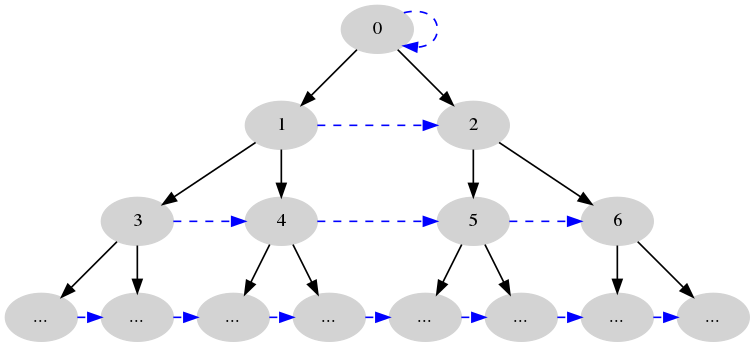
\includegraphics[width=8.5cm]{figures/chapter2/tdgraph.png}
  \caption[Complex decomposition of $\TAGraphRoot$ via task partitioning for a
  single robot.]{\label{fig:tdgraph} $\TDGraph$ is a complete binary tree
    formed by the black edges connecting the task nodes. Each $\phi_i$ is formed
    by connecting the nodes at height $i$ within $\TDGraph$ together with the
    blue edges. }
\end{figure}
%
Previous work~\cite{Harwell2018,Pini2011b,Frison2010,Ferrante2015} on task
partitioning divided the overall decomposable task $\TAGraphRoot$ into a sequence of
two interdependent atomic subtasks. We extend this decomposition by relaxing subtask
atomicity, allowing robots to partition subtasks into yet simpler subtasks
(Fig.~\ref{fig:tdgraph}). This \emph{recursive} task partitioning process results in
a \emph{complex} task decomposition graph~\cite{Korsah2013} with a \emph{multiplely
  decomposable} root task $\TAGraphRoot$. Recursive task partitioning results in a
complete binary tree, which we denote by $\TDGraph$, where $\TAGraphV{a}$ is the set
of all tasks in the tree, and $E_d$ is the set of connecting edges.

We consider a self-organizing swarm $\TheSwarm$ given an objective $\SwarmObjective$
to minimize the cost of repetitively completing $\TAGraphRoot$. Let
$\phi_a =\{v\in\TAGraphV{a}|height(v)=0,1,2,\ldots\}$ be the set of sets of vertices
with height $i$. Each ${\phi_a}\in{\Phi_a}$ is a topologically ordered task
decomposition within $\TDGraph$ (Fig.~\ref{fig:tdgraph}), and an equivalent means to
accomplish $\SwarmObjective$ (different \emph{functionalities} in the terminology
of~\cite{Williams2017}). From a natural standpoint, these decomposition sequences and
the tasks within them are analogous to the castes and observed task specialization
common among insects such as ants, bees, etc.~\cite{Duarte2011,Ferrante2015}.

Each $\ArbRobot\in\TheSwarm$ will execute a series of task allocations $a=1,\ldots,A$
(multiple task allocations may occur simultaneously, or involve a single robot at a
single instant in time); all robot task allocation decisions are independent. Each
time $\ArbRobot$ finishes a task ${v_f}\in{\TAGraphV{a-1}}$, it allocates a new task
${v_a}\in\TAGraphV{a}$.

During allocation at $T_{a}$, $\ArbRobot$ allocates a task $v_a$ from $\TAGraph{a}$
to execute next, minimizing a temporally varying cost function
$\CostFunc$. $\CostFunc$ represents the cost to $\ArbRobot$ of executing $v_a$
starting at time $t$. As $\ArbRobot$ allocates itself tasks over time, its allocation
history clearly forms a directed, weighted path within $\TAGraph{a}$. $\ArbRobot$
seeks a temporal path through $\TAGraph{a}$ that is optimal (of minimal
cost). Defining decision variables $x_{ij}\in{\{0, 1\}}$ indicating that task $j$ has
been allocated to robot $i$, and a utility $u_{ij}$ for the allocation $(i,j)$,
solving this problem optimally for $\TheSwarm$ is equivalent to solving the following
linear program for each allocation $a\in{A}$:
% [JRH] Should see if I can use one of the MRTA paper linear programs here--would be
% much stronger.
%
\begin{equation}
  \label{eqn:ta-linprog}
  \begin{array}{lc}
    \max &f(x_{ij},u_{ij}) \\
    \text{s.t.} &\sum\limits_{a\in{A}}\sum\limits_{j=1}^{|\TAGraphV{a}|}x_{ij} <= 1\\
    &\sum\limits_{i=1}^{|\TheSwarm|}x_{ij} <= T\\
  \end{array}
\end{equation}
%
with $f(x_{ij},u_{ij})$ a monotonically decreasing function. Each possible task is
assigned at most once, and robots can change their allocated task at most once per
timestep.
% -------------------------------------
\subsection{\glsfmtshort{stoch-n1} Task Allocation Space}\label{ssec:stoch-nbhd1-ta-space}
% -------------------------------------
To answer~\gls{RQ2.1}, we derive a task allocation space sensitive to task
decomposition graph richness. We induce a subgraph $\TAGraph{a}$ on $\TDGraph$
containing all tasks available to $\ArbRobot$ for allocation after it has finished
task ${v_f}\in\TAGraphV{A}$ at time $T_a$ by adding edges to $\TAGraphE{d}$ to form
$\TAGraphE{a}$ (union of solid and dotted edges in
Fig.~\ref{fig:tdgraph-reachable}). Formally:
%
\begin{equation}
  \TAGraphE{a} = \{e_{ji}~\forall~e_{ij}\in{\TAGraphE{d}}\}\cup\{e_{ij}~\forall~{v_i,v_j}\in\TAGraphV{a} : {i}\ne{j},sibling(v_i,v_j)\}
\end{equation}
%
$\TAGraph{a}$ (Fig.~\ref{fig:tdgraph-reachable}) then represents the union of
possible task allocations for each task ${v_f}\in\TAGraphV{A}$~$\ArbRobot$ could have
finished. We contextualize this task allocation graph around $v_f$ by defining its
\emph{allocation neighborhood}, restricting the tasks that can be allocated:
%
\begin{equation}
  \TAGraphE{nbhd} = \TAGraphE{a} \setminus \{{e}\in\TAGraphE{a} : dist(v_f,v)~\le~r_{nbhd}~\forall~{{v}\in\TAGraphV{A}}\}
\end{equation}
%
%That is,
$\TAGraphE{nbhd}$ induces a subgraph $\TAGraph{nbhd}$ on $\TAGraph{a}$ with
central vertex $v_f$ and radius $r_{nbhd}$. In this work we restrict our study to
$r_{nbhd}=1$; future work may further explore larger neighborhoods. Examples of the
three possible cases of this induced subgraph on $\TAGraph{a}$ with $r_{nbhd}=1$ are
shown in Fig.~\ref{fig:tdgraph-reachable}.
%
\begin{figure}[!htbp]
  \centering
  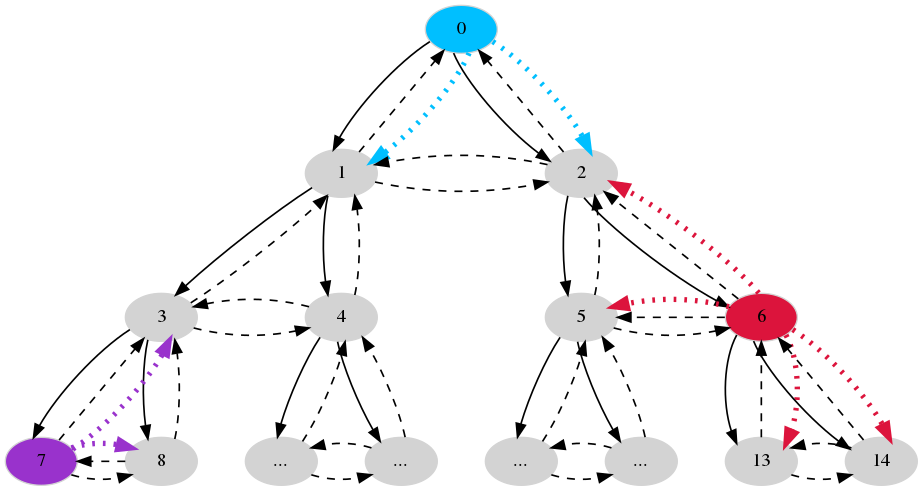
\includegraphics[width=8.5cm]{figures/chapter2/tdgraph-accessible.png}
  \caption[Task allocation neighborhoods $\TAGraph{nbhd}$ within
  $\TAGraph{a}$]{\label{fig:tdgraph-reachable}. Induced by $\TAGraphE{nbhd}$ for
    each $v_f\in\TAGraphV{a}$. A task is either the root (node 0, blue), a leaf
    node (node 7, purple), or neither (node 6, red). The three possible cases of
    allocation neighborhoods reachable from $v_f$ are shown via different
    colored edges.}
\end{figure}
% -----------------------------------
\subsection{\glsfmtshort{mat-opt} Task Allocation Space}\label{ssec:matopt-ta-space}
% -----------------------------------
We create a set of task allocation graphs $\TAGraph{|A|}$ (one for each task
allocation $\ArbRobot$ performs) connected through time via sets of directed edges
such that the connecting edges $\TAGraphE{a-1}$ from $\TAGraph{a-1}$ to $\TAGraph{a}$
each represent a possible task allocation decision leading from a specific
$v_f\in\TAGraphV{a-1}$ to any $v_a\in{\TAGraphV{a}}$. Given such connectivity, it is
clear that $\ArbRobot$ can choose its next task $v_{a}$ without restrictions
resulting from the neighborhood of $v_{a-1}$ (i.e., $r_{nbhd}=\infty$). Formally,
$\TAGraph{|A|}$ is defined by:
%
\begin{equation}
  \begin{array}{lc}
    \TAGraphV{|A|}=\bigcup\limits_{a=1}^{A}{\TAGraphV{a}} \\
    \TAGraphE{|A|}=\big(\bigcup\limits_{a=2}^{A-1}\{{v_{a-1}}\in{V_{a-1}},{v_{a}}\in{V_{a}} : e_{v_{a-1},v_{a}}\}\big)
  \end{array}
\end{equation}
%
That is, for all
$a=2,\ldots,A, {deg}^{-}(v)={deg}^{+}(v)=|\TAGraphV{a}|~\forall~{v\in\TAGraphV{a}}$.

Using the notation of~\cite{Williams2017}, we define an allocation
${v}\in\TAGraphV{|A|}$ more formally as a triplet $(s,v_{j},\phi_{k})$, read as
``robot $s$ performs task $v_j$ to for $\phi_k$''. Then, $\SwarmObjective$ can be
more precisely defined as
$\SwarmObjective\subseteq\{(v_j,\phi_k) |
v_j\in{\TAGraphV{|A|},\phi_k\in\Phi_{|A|}}\}$. That is, a robot allocates a task
$v_j\in{\TAGraphV{a}}$ from $\phi_k\in\Phi_a$ in order to help complete
$\SwarmObjective$ by performing a task from the task sequence at height $k$ within
$\TAGraph{|A|}$. We assign an independent set $\IndSets_{\ArbRobot}$ to each
$\ArbRobot\in\TheSwarm$, containing sets of triplets $\{(s,v_{j},\phi_{k})\}$ which
are the feasible sets of functionality-requirement~\cite{Williams2017}
allocations. Then,
$\ArbRobotMatroid\in\mathbb{M},\ArbRobotMatroid=(\TAGraphV{|A|},\IndSets_{\ArbRobot})$
are matroids containing the set of maximal independent sets for each
$\IndSets_{\ArbRobot}$. From~\cite{Williams2017}, an optimal task allocation policy
can be obtained from the intersection of these matroids (a reframing of
Eqn.~\eqref{eqn:ta-linprog}).

We now set our matroid optimality constraints and prove that $\ArbRobotMatroid$
satisfies the matroid
properties~\ref{prop:matroid1},~\ref{prop:matroid2},~\ref{prop:matroid3}:

\begin{enumerate}
\item {\emph{$\CostFunc$ monotonicity and accuracy}. We assume $\CostFunc$ is a
    monotonically increasing function which accurately estimates the cost of
    performing a task $v$ starting at time $t$, and that this accuracy is maintained
    regardless of the task allocations chosen. That is, while a task allocation at
    $T_a$ might affect future task costs at time $T_{a'}$, those cost changes do not
    violate monotonicity. By our definition, $-\CostFunc$ is a \emph{sub-modular
      monotone} function~\cite{Williams2017}.

    Environments such as large-scale robotics warehouses are well modeled by cost
    functions of this type. For example, data about how long it takes to find an
    object of a specific type and bring it to a specific location are well known, and
    provide excellent estimates of the execution time for tasks. However,
    sensor/actuator error can still cause the theoretically collision-free paths to
    not be collision free in practice, thus increasing actual task execution times
    beyond estimates, but not to reduce them. }
\item {\emph{Task allocation independence}. While a task chosen by $\ArbRobot$ might
    affect the future task cost estimates of another robot $\ArbRobotTwo$, such
    effects will not change $\ArbRobotTwo$'s allocation decisions, due to $\CostFunc$
    monotonicity and submodularity. }
\item {\emph{Task allocation frequency}. We assume $\ArbRobot$ can abort its current
    task and allocate a new one at any point in time. }
\item {\emph{Task Switching Cost}. We assume $\ArbRobot$ can switch tasks without
    cost, or equivalently, with equal cost. Without loss of generality, task
    switching costs can be encoded in $\CostFunc$.}
\item {\emph{Temporal precedence constraint satisfaction}: All constraints for a task
    $v_j$ are satisfied when $\ArbRobot$ allocates itself $v_j$. That is, for a task
    $v_j$ at position $j$ within a task sequence $\phi_i$, other robots have already
    completed all tasks ${v_{0}}\ldots{v_{j-1}}$ in the specific instantiation of the
    sequence. This is a restatement of the assumptions of~\cite{Frison2010,Dahl2009},
    in which task independence is unaffected by group dynamics, and effectively
    removes task dependencies from $\TAGraph{a}$.  This is a necessary assumption for
    proving $\ArbRobotMatroid$ is a graphic matroid, because graphic matroids cannot
    contain cycles, and edges between tasks within the same $\TAGraphV{a}$ trivial
    form cycles between the allocations performed at $T_a$ and $T_{a+1}$. }
\end{enumerate}

We wish to create an independence system $\IndSets_{\ArbRobot}$ over $\TAGraphV{|A|}$
and, furthermore, show that $\ArbRobotMatroid=(\TAGraphV{|A|},\IndSets_{\ArbRobot})$
is a matroid. We define $\IndSets_{\ArbRobot}$ as:
% [LL] From https://math.stackexchange.com/a/3312756/357287.
\begin{equation}\label{eqn:indsystem}
  \IndSets_{\ArbRobot} = \{I: I \subset \TAGraphV{|A|}, |I \cap \TAGraphV{a}| \le 1 ~\forall~{a =
    1,\ldots,A} \}
\end{equation}
%
\begin{figure}[!htbp]
  \centering
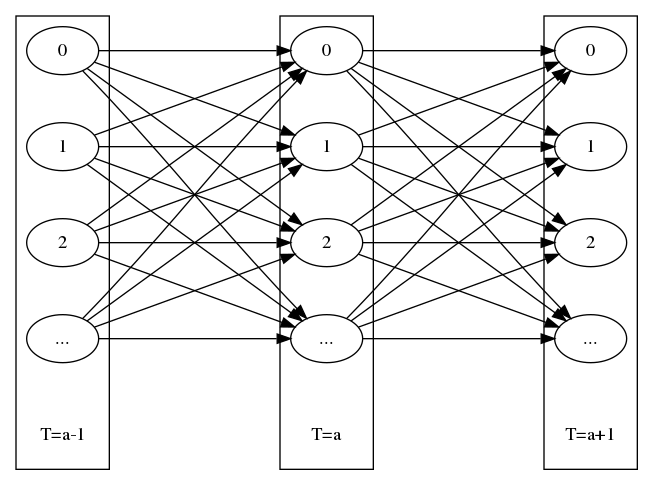
\includegraphics[width=5cm]{figures/chapter2/temporal-ta-graph.png}
\caption[Unrolled task allocation graph
$\TAGraph{|A|}$]{\label{fig:temporal-ta-graph} Shown for arbitrary task
  allocation times $a-1,a,a+1$.}
\end{figure}
%
$\IndSets_{\ArbRobot}$ consists of every set of task allocation decisions that
$\ArbRobot$ can make ($\ArbRobot$ cannot choose more than one task during a single
allocation). Since tasks take varying amounts of time, task allocation decisions can
occur at \emph{any} $1\le{t}\le{T}$. Depending on the previous decisions made (i.e.,
the members of a particular ${X}\in{\IndSets_{\ArbRobot}}$), at some time $t^{*}$
another decision will be made and another vertex added to $X$ (i.e., a robot aborts
its current task and starts the new task, which had \emph{smaller} cost than the
remaining portion of its current task). For another
${Y}\in{\IndSets_{\ArbRobot}},{X}\ne{Y}$, $t^{*}$ will occur while $\ArbRobot$ is
executing a task, and 0 tasks from $\TAGraph{t^{*}}$ will be added to $Y$ (if the new
task does not have a lower cost estimate than the remaining part of $\ArbRobot$'s
current task). Effectively, robots perform task allocation each timestep, choosing to
continue their current task or to abort it and choose a new one, depending on which
they think will have smaller cost and finish first.

To prove $\IndSets_{\ArbRobot}$ is an independence system, we now
prove~\ref{prop:matroid1}, ~\ref{prop:matroid2}. \ref{prop:matroid1} is true by
construction, as $\TAGraphV{|A|}=\emptyset$ is admissable under
Eqn.~\eqref{eqn:indsystem}.~\ref{prop:matroid2} is also satisfied by construction,
because we defined $\IndSets_{\ArbRobot}$ so that for every
${X}\in{\IndSets_{\ArbRobot}}$, no pair of elements in $X$ are a part of the same
$\TAGraphV{a}$, by Eqn.~\eqref{eqn:indsystem}. Thus, for a subset of $X$, which has
\textit{fewer} elements, it would also be true that no pair of elements would be a
part of the same $\TAGraphV{a}$. Since $\IndSets_{\ArbRobot}$ is an independence
system, any ${I}\in\IndSets_{\ArbRobot}$ is an \emph{independent set}.

Finally, we must prove~\ref{prop:matroid3} for $\IndSets_{\ArbRobot}$ for any
$\ArbRobot\in\TheSwarm$, in a similar manner to~\cite{Williams2017}: for any two sets
of task allocation decisions $\{X\},\{Y\}$, if $|X| < |Y|$, we can take an allocation
decision from $Y$ and add it to $X$ and still have a valid independent set. Since $X$
and $Y$ contain at most one element per allocation time, then we must have
$|X|<|Y|\le{A}$, and therefore there must be least one time $T_{a^{*}}$ for which
$|X \cap \TAGraphV{a^*}| = 0$ and $|Y \cap \TAGraphV{a^*}| = 1$. Then we know
$Y \cap \TAGraphV{a^*} \subseteq{Y} \setminus{X}$ such that
$X \cup \{Y \cap \TAGraphV{a^*}\} \subset \IndSets_{\ArbRobot}$. In other words,
since $|Y| > |X|$, it must have done an allocation at a time when $X$ did not, and
this allocation can be added to $X$ to form a new independent set.

This concludes the proof of~\ref{prop:matroid3}, and therefore
$\ArbRobotMatroid=(\TAGraphV{|A|},\IndSets_{\ArbRobot})$ for all
$\ArbRobotMatroid\in{\mathbb{M}}$ are matroids.

\section{Task Allocation Methods}
\subsection{\glsfmtshort{stoch-n1} Task Allocation Method}\label{ssec:stoch-nbhd1-method}
%
\begin{algorithm}[htb]
  \caption{\gls{stoch-n1}()}
  \textbf{INPUT:}$\beta$,$v_f$ \;
  \textbf{OUTPUT:}$\beta',v_{a}$ \;
  \begin{algorithmic}[1]\label{alg:ta-stoch-nbhd}
    \IF{$v_f = \beta_{0}$} \label{alg:ta-stoch-nbhd-tab-start}
    \STATE$\beta'\gets$ SwitchContext($\beta, \beta_{parent(v_f)}$)
    \ELSE%
    \STATE$\beta'\gets$ SwitchContext($\beta, \beta_{v_f}$)
    \ENDIF\label{alg:ta-stoch-nbhd-tab-end}%
    \IF{EmployPartitioning($\beta'$)}\label{alg:ta-stoch-nbhd-context-start}
    \RETURN{$\beta'$, $ChooseChild(\beta'$)}
    \ELSE%
    \RETURN{$\beta'$,$\beta'_{0}$}
    \ENDIF\label{alg:ta-stoch-nbhd-context-end}%
  \end{algorithmic}
\end{algorithm}
%
We define a method capable of task allocation in each of the 3 cases for
$\TAGraph{nbhd}$ from Fig.~\ref{fig:tdgraph-foraging} in
Algorithm~\ref{alg:ta-stoch-nbhd}. \newline $EmployPartitioning()$ and
$ChooseChild()$ are the task partitioning and subtask selection methods
from~\cite{Harwell2018}, and $\beta_i$ is the \emph{Task Allocation Block} (TAB), a
binary tree consisting of a root partitionable task $\beta_{00}$ and its two
subtasks, $\beta_{01},\beta_{02}$. We use numerical subscripts $ij$ attached to
$\beta_{ij}$ to denote the $j$th task within a TAB rooted at vertex $i$ (we use a
left-to-right numbering scheme, as depicted in Fig.~\ref{fig:tdgraph}). In previous
work, there was only a single TAB, $\beta_0=\TAGraphNBHD$ with $|\TAGraphV{a}| = 3$.

Lines~\ref{alg:ta-stoch-nbhd-context-start}-\ref{alg:ta-stoch-nbhd-context-end} of
Algorithm~\ref{alg:ta-stoch-nbhd} are unambiguous if and only if
$|\TAGraphV{a}| = 3$, because for such graphs, only a single partitionable task
exists, and all partitioning decisions are rooted at that node, regardless of
$v_f$. However, for ${v_f}\in\TAGraphV{a}, |\TAGraphV{a}| > 3$ that are neither the
root or a leaf node, ambiguity exists in \emph{which} node to consider as the
pseudo-root for the purposes of partitioning (see
Fig.~\ref{fig:tdgraph-TABs}). Should the pseudo-root be $parent(v_f)$, considering
$v_f$ to be a pseudo-leaf node within a 3 node graph rooted at $parent(v_f)$? Or
should it be $v_f$, considering $v_f$ as the root node of a 3 node tree encompassing
$v_f$ and its two children?  We solve the ambiguity of \emph{which} node to consider
as the pseudo root by allowing multiple $\beta\subset{\TAGraph{a}}$; every vertex $v$
that is not a root or leaf is both the root of a $\beta$ rooted at $v$, and a leaf
within a $\beta$ rooted at $parent(v)$ (see Fig.~\ref{fig:tdgraph-TABs}). With this
extended TAB definition, we now consider the question of \emph{how} $\ArbRobot$
should update the TAB associated with $v_f$ (the definition of the $SwitchContext()$
function).
%
\begin{figure}[!htbp]
  \centering
  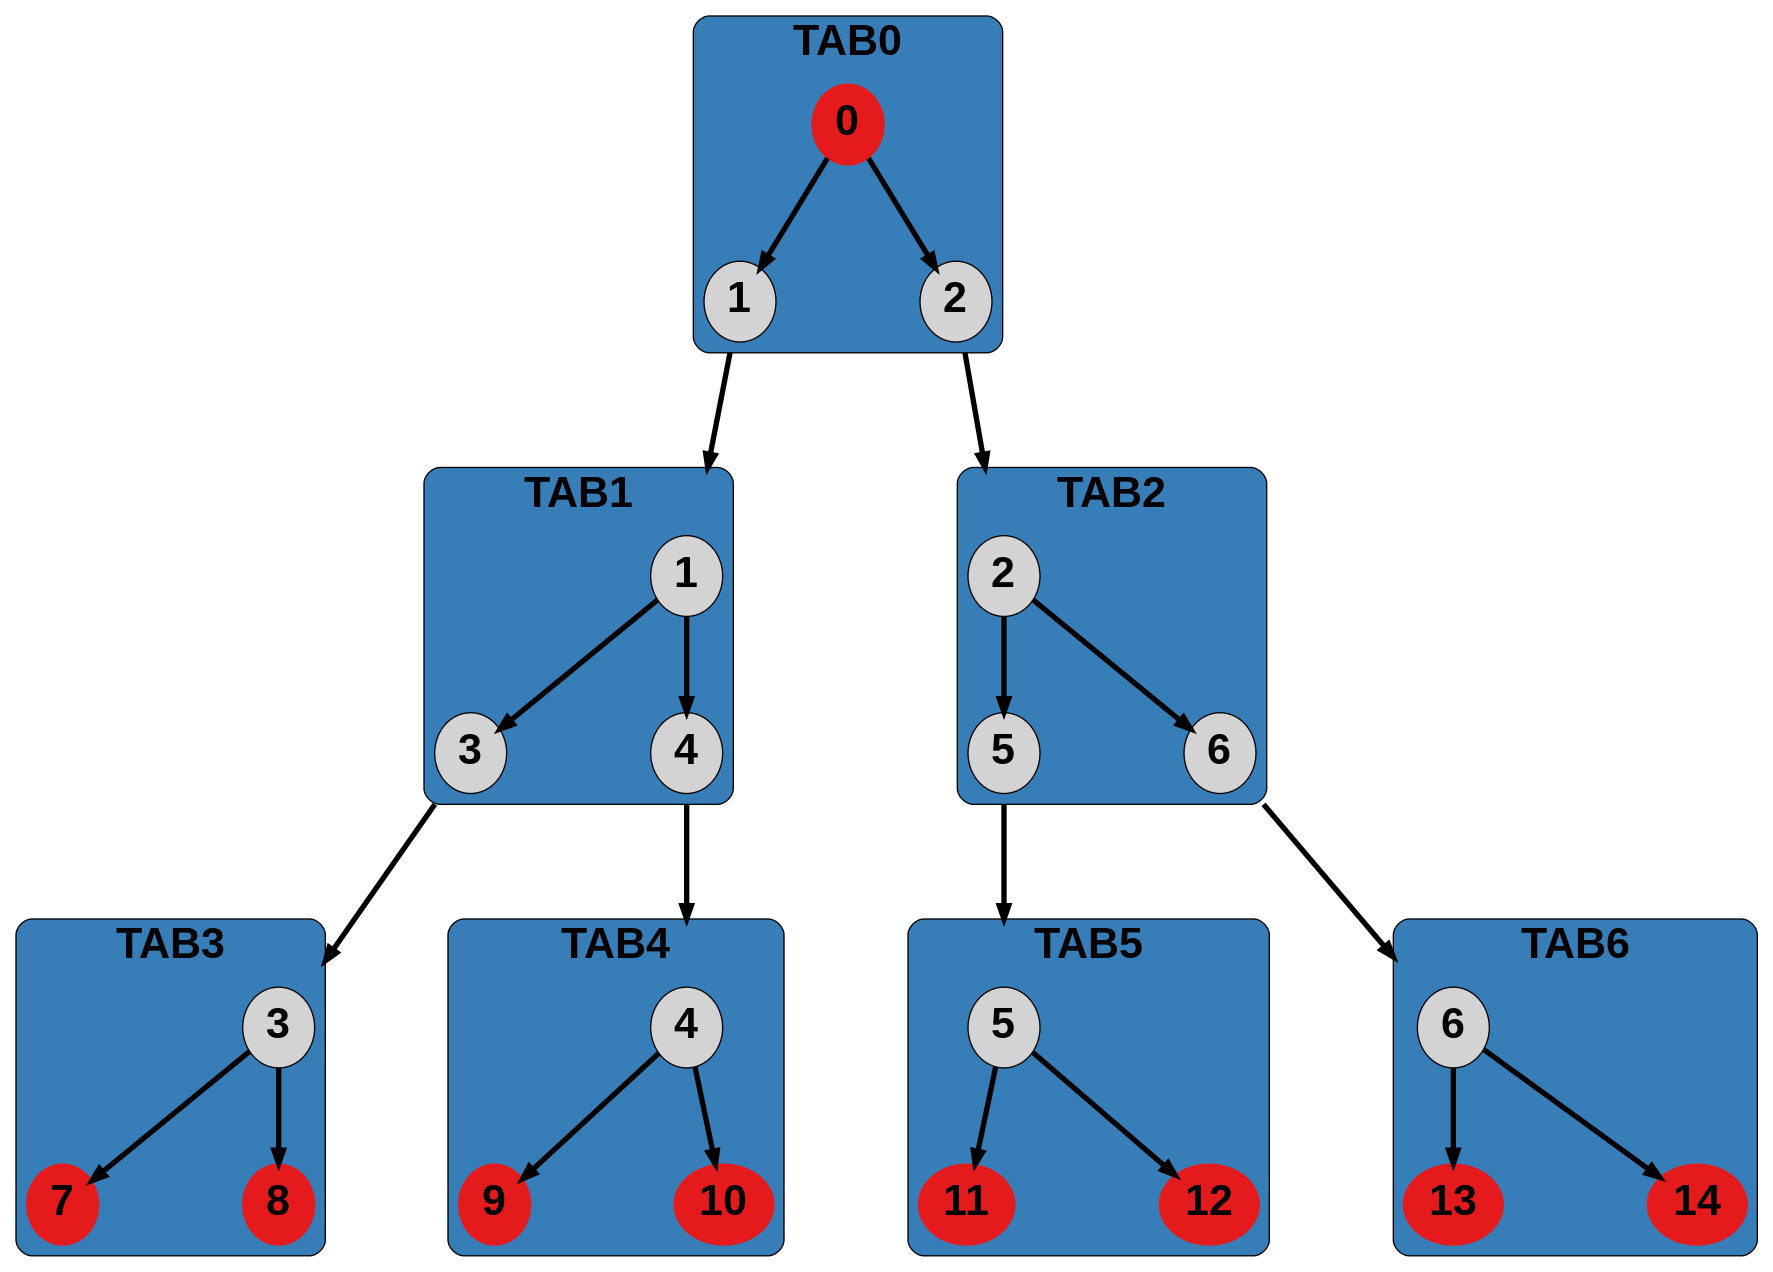
\includegraphics[width=7cm]{figures/chapter2/tdgraph-tabs.png}
  \caption[Task Allocation Contexts (TABs) within
  $\TAGraph{a}$.]{\label{fig:tdgraph-TABs} $v_f$ with unambiguous partition
    points in red (root and leaf nodes), and ambiguous partition points in
    gold.}
\end{figure}
%
\smallskip\smallskip\smallskip
%
From the task decomposition graph structure, each subtask $(\beta_{i1},${}
$\beta_{i2})$ is half of the work of $\beta_{i0}$, it should therefore have half the
cost under $\CostFunc$. The further this ratio becomes unbalanced, the more likely
that stochastic variances in the swarm and/or environment will cause tasks to
unexpectedly take longer, and the less reliable task estimates should be
considered. So a robot attempting to stochastically minimize the cost of the tasks
they choose should change the current $\beta_{i}$ to a different $\beta_{j}$ within
$\TAGraph{a}$, depending on how ``balanced'' task cost estimates are between
different $\beta\subset{\TAGraph{a}}$; that is, how close the cost estimate for
$\hat{\beta_{i0}}$ is to the sum of the cost estimates of its subtasks
$(\hat{\beta_{i1}} + \hat{\beta_{i2}})$. We formalize this intuition in the following
equations, which comprise the essence of $SwitchContext()$:

\begin{equation}\label{eqn:TAB-sw-theta}
  \theta_{\beta}(\beta_i,\beta_j) = \Omega_{\beta_r}\Big(\frac{|\hat{\beta_{i0}} -
    (\hat{\beta_{i1}} + \hat{\beta_{i2}})| / \hat{\beta_{i0}}}
  {|\hat{\beta_{j0}} - (\hat{\beta_{j1}} +
      \hat{\beta_{j2}})| / \hat{\beta_{j0}}} -\Omega_{\beta_o}\Big)
\end{equation}

\begin{equation}\label{eqn:TAB-sw}
  P_{\beta_{sw}}(\beta_i,\beta_j) = \frac{1}{1 + e^{-\theta_{\beta}(\beta_i,\beta_j)}}
\end{equation}

Where $\Omega_{\beta_r}$ is the reactivity of the logistic function, and
$\Omega_{\beta_o}$ is the offset. In the degenerate case in which the ratios are
exactly equal, $P_{\beta_{sw}}$ is 0.5 (we choose $\Omega_{\beta_o} = 1.0$ in this
work). Using Eqn.~\eqref{eqn:TAB-sw}, and our extended TAB definition, a robot is
constrained in its choices to update $\beta_i$ by the structure of $\TAGraph{a}$ to
$\{\{\beta_i\}\cup{\{\beta_j : v_f = \beta_{j1,j2}\}}\}$ if $v_f=\beta_{i0}$, and
$\{\{\beta_i\}\cup{\{\beta_j : v_f = \beta_{j0}}\}\}$ otherwise.

The \gls{stoch-n1} algorithm (Algorithm~\ref{alg:ta-stoch-nbhd}) extends the task
allocation algorithms from previous
work~\cite{Pini2011b,Brutschy2014,Ferrante2015,Frison2010,Harwell2018}
(lines~\ref{alg:ta-stoch-nbhd-context-start}-\ref{alg:ta-stoch-nbhd-context-end})
with lines~\ref{alg:ta-stoch-nbhd-tab-start}-\ref{alg:ta-stoch-nbhd-tab-end}, solving
the problem of task partition node ambiguity. It realizes $\TAGraph{nbhd}$ with
$r_{nbhd}=1$, because all $\beta\in\TAGraph{nbhd}$ have radius 1, and therefore $v_a$
will be a distance of at most 1 from $v_f$. It is therefore well suited to
investigate the effect of $\TAGraph{a}$ richness on emergent intelligence. It
approximately solves Eqn.~\eqref{eqn:ta-linprog} via stochastic greedy allocation for
a single $a\in{A}$ at a time, not considering future allocations, and does not have
any guarantees of optimality.
%
\subsection{\glsfmtshort{mat-opt} Task Allocation Method}\label{ssec:matopt-method}
%
$\ArbRobot$ seeks an optimal path (measured by $\CostFunc$) between $v_{a1}$ and
$v_{aA}$, which belong to $\TAGraph{1}$ and $\TAGraph{A}$, respectively. We define a
global greedy algorithm $GG$ capable of finding the lowest cost path between $v_{a1}$
and $v_{a2}$ by determining the best decision for a robot to take at any time. Let
$\hat{v_{a}}$ be the robot's cost estimate of a task ${v_{a}}\in\TAGraphV{a}$ using
our cost measure $\CostFunc$ at time $T_a$. The algorithm begins with
$F_{0}=\emptyset$, and iteratively selects at task allocation time $T_1$ the element
${v_a}\in\TAGraphV{1}$ independent from $F_{a-1}$ maximizing $-C(v_a,t)$:

% [JRH] Can possibly cite the 'local optimal' part of the algorithm they run as being
% what each robot in the swarm runs, saying we think the swarm emergent intelligence
% can make up for the lack of communication, formal optimization, etc. that happens
% in that work.
\begin{equation}
F_{a} = F_{a-1} \bigcup\Big\{\argmax\limits_{v_a: F_{i-1}\cup\{v_a\}\in{\IndSets_{\ArbRobot}}}-C(v_a,t|F_{a-1})\Big\}
\end{equation}

It follows that the $GG$ algorithm gives the optimal decision path for
$\ArbRobot$~\cite{Oxley2006}. The path is not guaranteed to be unique; all optimal
paths will have the same overall cost and cardinality due to~\ref{prop:matroid3}.

In real SR systems, a global greedy algorithm is not possible in general: environment
conditions can change, robots can enter/leave an operating area, robots can fail,
sensor/actuator errors can result in unpredictable congestion. All these events
affect the optimal decision path, and cannot be known \emph{a priori}.

We now define a local greedy algorithm ($LG$) for determining what decision a robot
should make without any information about future costs, and show that this algorithm
gives the same result as $GG$. The $LG$ algorithm begins with an empty set $F_{LG}$,
and at each task allocation $a=1,\ldots,A$, it adds
$\argmax_{v_{a}\in{\TAGraphV{a}}}{\hat{v_a}}$ to $F_{LG}$ (accurate task selections
ensured by accurate and monotonically increasing task cost estimates).

We prove that $LG$ gives the same result as $GG$ with a proof by
contradiction. Assume that $LG$ does worse than $GG$. That is,
$\sum_{{v}\in{F_{LG}}} \hat{v} < \sum_{v\in{F_{GG}}} \hat{v}$. Note that since
$F_{GG}$ is maximally independent, and LG chooses exactly one task at each
allocation, both $F_{GG}$ and $F_{LG}$ have exactly one task from each $V_{a}$. Thus,
in order for $\sum_{v\in{F_{LG}}} \hat{v} < \sum_{v\in{F_{GG}}} \hat{v}$ to be true,
it must also be true that there exists some task allocation time $T_{a^*}$ for which
the task chosen by $GG$ from $V_{a^*}$ has a smaller estimated cost than the task
chosen by $LG$ from $V_{a*}$. However, this is impossible, because we have defined
$LG$ to take the task with the least cost from each $V_a$. Thus, since $LG$ cannot do
worse than $GG$, it must also be optimal.~\qed

\subsection{Experimental Setup}\label{sec:exp-and-results}


\section{Discussion}

We observe in Fig.~\ref{fig:DS-self-org} that the self-organization measure we employ
(derived by~\cite{Harwell2019a}) is sensitive to the task allocation method, and that
considerable self-organization emerges, in comparison to the baseline random
allocation method. However, in this work we have only established a rough correlation
between emergent intelligence and performance, as we see that even though swarms
using random task allocation still outperform more ``intelligent'' methods such as
UCB1 in many cases. One would expect that the \gls{mat-opt} and $\epsilon$-greedy methods,
even without optimality constraints in place (as in this case), would do better than
randomized allocations.

Comparing the heatmaps in Fig.~\ref{fig:DS-perf} across all methods, it is clear that
the richness of the task allocation graph positively affects self organization, which
we believe is due to the swarm's increased ability to dynamically adapt to changing
traffic flows as time progresses. From this we can answer~\gls{RQ2.1} and
conclude that (1) task decomposition graph richness has an important and measurable
effect on the emergent intelligence of a swarm, (2) more complex task decomposition
graphs result in higher levels of emergent intelligence, (3) swarm emergent
intelligence is positively correlated with performance.

Within Fig.~\ref{fig:DS-relaxation-depth1} (compound task decomposition graph), we
see empirical evidence that our matroid optimality constraints and method of
enforcement were valid through the consistent performance drops observed across
scales for \gls{mat-opt} and $\epsilon$-greedy. Examining
Fig.~\ref{fig:DS-relaxation-depth2}, we see a general lack of trends between
performance under relaxation vs.~under constraints, for all tested methods, which we
attribute to pthe higher levels of swarm intelligence present via the complex task
decomposition graph. That is, the lack of trends is due to collective learning of the
graph \emph{structure}, rather than graph \emph{content}, which gives rise to higher
levels of swarm intelligence, and the richer structure of the complex decomposition
graph overwhelms the effect of the optimality constraints.

For both types of decomposition graphs, the \gls{mat-opt} method was \emph{not}
the optimal method, even under constraints, though we do observe the largest
performance boost of all the tested methods under perfect
information. \gls{mat-opt} ignores task decomposition graph structure, and
assumes independent tasks, which is shown to be an invalid assumption. In
addition, from Fig.~\ref{fig:DS-perf} and the performance drops in
Fig.~\ref{fig:DS-relaxation-depth1}, Fig.~\ref{fig:DS-relaxation-depth2},
\gls{stoch-n1} performs the best under both imperfect and perfect information,
though it experiences performance drops, rather than increases, under perfect
information. Random performed the second best in many cases, though it was
outperformed by UCB1 in some cases. From these observations we can
answer~\ref{research-Q2}, concluding that from a task allocation perspective,
swarm intelligence arises out collective learning of the structure and
connectivity of the graph, rather than collective learning of the graph content
(tasks and task costs), and that task dependencies cannot be ignored even in
independent task allocation decisions made by individual robots.

From this discussion, it is clear that leveraging emergent intelligence is crucial in
establishing (practically) optimal task allocation policies in robot swarms, and that
maximally performing solutions (possibly without optimality guarantees) need to
incorporate stochasticity in order to mitigate (or exploit) their inherent
randomness. We have also shown that there are formal task allocation methods (UCB1)
well suited to traditional typical environments when perfect information is not
available. Finally, our \gls{mat-opt} results suggest that emergent intelligence has the
potential, under the right conditions, to work synergistically with theoretical
models, if task independence is guaranteed.
%
\section{Conclusions and Future Work}\label{sec:conclusions}
%
We have investigated the effect that the richness of task decomposition graph has on
emergent swarm intelligence. We derived compound task decomposition graphs enabling
swarms to utilize existing caches, and complex task decomposition graphs enabling
them to create/destroy caches. We have shown that task decomposition graph richness
is positively correlated with swarm emergent intelligence and performance for many
task allocation methods in an object gathering task. We have further studied the
emergence of swarm intelligence as it relates to task decomposition graphs, showing
that it arises out of learning and exploitation of graph structure, rather than graph
context (task costs of nodes). Future work should investigate the conditions under
which emergent swarm intelligence can be made to work synergistically with
theoretical models. More work is also needed to refine the relationship between
emergent intelligence and performance. In order to facilitate future research and
collaboration, the code used for this research is open source, and can be found at
https://github.com/swarm-robotics.
